\section{Caracter\'isticas principales}        
\begin{frame}
    \frametitle{Caracter\'isticas principales}
%    \framesubtitle{Caracter\'isticas principales}
    
    \begin{block}{}
        \begin{columns}
        
            \column{0.3\textwidth}
            \textcolor{red}{\textbf{F}}ield \\ 
            \textcolor{red}{\textbf{O}}peration \\
            \textcolor{red}{\textbf{A}}nd \\
            \textcolor{red}{\textbf{M}}anipulation
            
%            \column{0.1\textwidth}
%            $$\Longrightarrow$$
            
            \column{0.6\textwidth}
            \centering
            Conjunto libre de bibliotecas de C++ para soluci\'on de ecuaciones diferenciales desarrollado por OpenCFD Ltd.
        \end{columns}                        
    \end{block}
        

    \begin{columns}
    
        \column{0.4\textwidth}
        \begin{block}{Aplicaciones}
            \begin{itemize}
                \item Fluidos compresibles
                \item Fluidos incompresibles
                \item Flujos multifase
                \item Transferencia de calor
                \item Din\'amica molecular
                \item Electromagnetismo
            \end{itemize}
        \end{block}
        
        \column{0.4\textwidth}
        \begin{exampleblock}{}
            \centering
            M\'etodo de vol\'umenes finitos en 3 dimensiones
        \end{exampleblock}        
        
        \begin{block}{}
            \centering
            Elementos poli\'edricos con cantidad ilimitada de caras
        \end{block}  
        
        \begin{block}{}
            \centering
            Gran flexibilidad en la descripci\'on geom\'etrica del dominio
        \end{block}
        
    \end{columns}        
    
\end{frame}




%---------------------------------------------------------------------------------------------------------------%
\begin{frame}
    \frametitle{Caracter\'isticas principales}
%    \framesubtitle{Caracter\'isticas principales}
    

    \begin{figure}
        \centering
        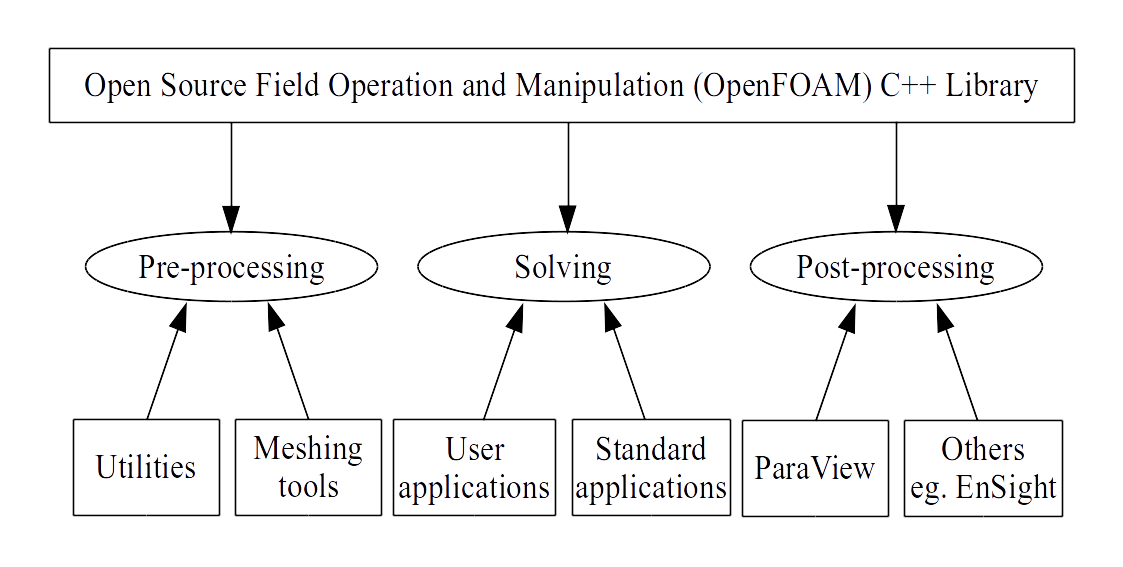
\includegraphics[scale=0.4]{Imagenes/diagrama}
    \end{figure}
    
    \begin{exampleblock}{}
        \footnotesize
        \begin{itemize}
            \item C\'odigo libre y gratuito, bajo licencia GNU.
            \item Los usuarios pueden crear sus propias aplicaciones y utilidades.
        \end{itemize} 
    \end{exampleblock}
    
\end{frame}





%---------------------------------------------------------------------------------------------------------------%
\begin{frame}
    \frametitle{Caracter\'isticas principales}
%    \framesubtitle{Caracter\'isticas principales}
    
%    Estructura de archivos
    \begin{figure}
        \centering
        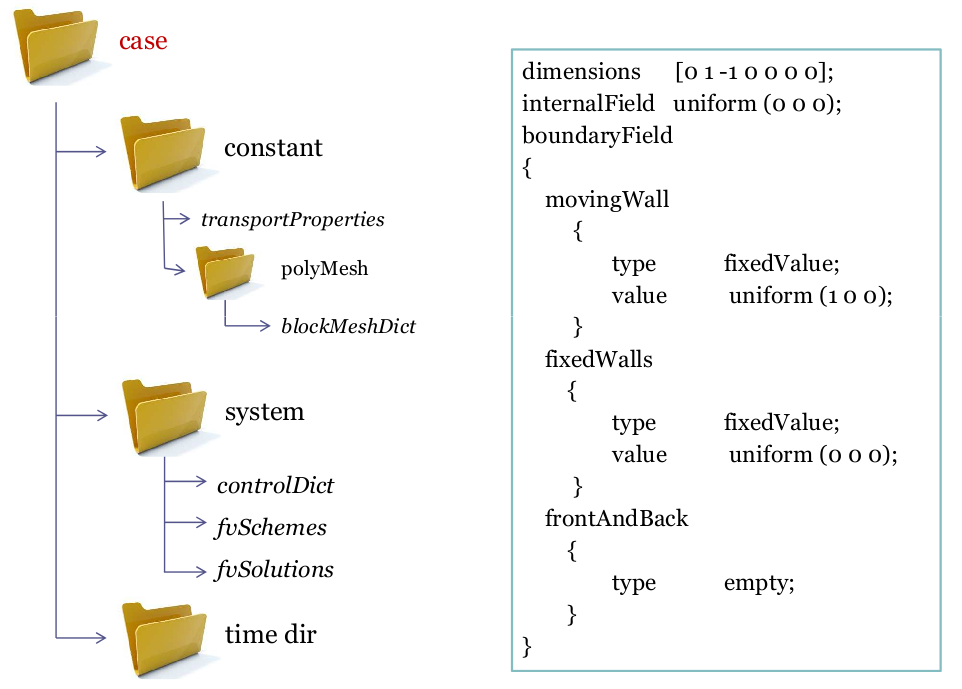
\includegraphics[scale=0.3]{Imagenes/file_structure}
    \end{figure}
    
\end{frame}


%---------------------------------------------------------------------------------------------------------------%
